\section{本章小结}

形而上方面,本章介绍了数学的思维范式——演绎法,在以后的学习过程中需要不断加深认识。形而下方面,本章介绍了逻辑的基本知识。集合和逻辑用语是现代数学的语言基础。本章定义了一些数学符号,如$\cap ,\cup ,\in ,\forall ,\exists $,这些符号使得数学语言脱离了自然语言,去除了自然语言的模糊性,让数学更加清晰精准。随着学习的深入,我们会定义更多的数学符号,记住,数学符号就是为了精确、准确、无歧义地表述。

我们再用数学判断命题或计算某个值时,往往使用“定理—定义—性质”这个步骤。如计算下面$\bigtriangleup ABC$的角$\alpha $,我们可以按如下步骤:
\begin{enumerate}
    \item 用定理证明$\bigtriangleup ABC$和$\bigtriangleup abc$相似;
    \item 用性质得到$\alpha =60^\circ$。
\end{enumerate}

\begin{figure}[h]
\centering
\begin{minipage}{.49\textwidth}
\centering
\begin{tikzpicture}[line join=round, scale=1]
\coordinate[label=above:{$A$}] (A) at (0.5,1);
\coordinate[label=left: {$B$}] (B) at (-1,0);
\coordinate[label=right:{$C$}] (C) at (1,0);
\draw[thick] (A)--(B)--(C)--(A);
\pic["$\alpha $",draw,angle radius=0.5cm,angle eccentricity=1.5] {angle=A--C--B};
\end{tikzpicture}
\end{minipage}
\begin{minipage}{.49\textwidth}
\centering
\begin{tikzpicture}[line join=round, scale=1.5]
\coordinate[label=above:{$a$}] (A) at (0.5,1);
\coordinate[label=left: {$b$}] (B) at (-1,0);
\coordinate[label=right:{$c$}] (C) at (1,0);
\draw[thick] (A)--(B)--(C)--(A);
\pic["$\pi /3$",draw,angle radius=0.5cm,angle eccentricity=1.8] {angle=A--C--B};
\end{tikzpicture}
\end{minipage}
\end{figure}

定义是逻辑起点,也是我们围绕的中心,是我们学习数学时的重中之重。定理是用来快速判断是否符合定义,让我们在逻辑上对定义有更深刻的认识。性质则是用来得到我们想要的结果。

~

\begin{example}[综合运用8,难度:$\star $]
已知
\begin{align*}
&A=\left\{ \left( x,y \right) \middle| 2x-y=0 \right\} \\
&B=\left\{ \left( x,y \right) \middle| 3x+y=0 \right\} \\
&C=\left\{ \left( x,y \right) \middle| 2x-y=3 \right\}
\end{align*}
求$A\cap B,A\cap C$,并解释它们的几何意义。
\end{example}

解:

\begin{align*}
&A\cap B=\left\{ \left( x,y \right) \middle| \left\{ \begin{array}{c}
	2x-y=0\\
	3x+y=0\\
\end{array} \right. \right\} \\
&A\cap C=\left\{ \left( x,y \right) \middle| \left\{ \begin{array}{c}
	2x-y=0\\
	2x-y=3\\
\end{array} \right. \right\}
\end{align*}

$A,B,C$几何上均表示平面的直线,$A\cap B$表示点即在直线$A$上也在直线$B$上,所以是它们的交点。不难发现,$A\cap B$是有交点的,但$A\cap C$表示两条平行线,没有交点。
\begin{figure}[ht]
\centering
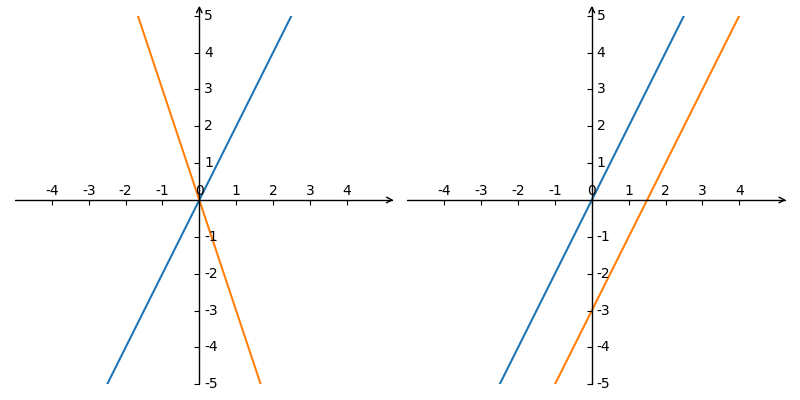
\includegraphics[height=4cm]{1.6-2.png}
\end{figure}

\begin{tcolorbox}
该题注意数形结合。
\end{tcolorbox}

~

\begin{example}[拓广探索12(2),难度:$\star \star \star $]
如图,在$\bigtriangleup ABC$中,$AD,BE,CF$分别为边$BC,AC,AB$上的高,证明$AD,BE,CF$交于点$O$。
\end{example}

解一,使用替换概念的思路:

在中学平面几何里面,我们学到过三角形有4个心:
\begin{itemize}
    \item 垂心,三角形三条高的交点;
    \item 重心,三角形三条中线的交点;
    \item 外心,三角形三条边的中垂线的交点,也是三角形外接圆的圆心;
    \item 内心,三角形三条角平分线的交点,也是三角形内切圆的圆心。
\end{itemize}
显然,在这里面最接近于三条高交点的是外心。于是,我们构建$\bigtriangleup A'B'C'$,使得$A'B'\parallel AB,A'C'\parallel AC,B'C'\parallel BC$。不难证明,$AD,BE,CF$为$\bigtriangleup A'B'C'$的中垂线,必交于一点,证毕。

\begin{figure}[h]
\centering
\begin{tikzpicture}[line join=round, scale=2.5]
\pgfmathparse{0.6/2.5}
\coordinate[label=left:       {$C'$}] (C') at (-1,0);
\coordinate[label=right:      {$B'$}] (B') at (1,0);
\coordinate[label=below:      {$A'$}] (A') at (-0.2,-1.3);
\coordinate[label=above:      {$A$}]  (A)  at ($(C')!0.5!(B')$);
\coordinate[label=below left: {$B$}]  (B)  at ($(C')!0.5!(A')$);
\coordinate[label=below right:{$C$}]  (C)  at ($(A')!0.5!(B')$);
\coordinate[label=below:      {$D$}]  (D)  at ($(B)!(A)!(C)$);
\coordinate[label=above right:{$E$}]  (E)  at ($(A)!(B)!(C)$);
\coordinate[label=above left: {$F$}]  (F)  at ($(A)!(C)!(B)$);
\draw[thick,dashed,red] (A')--(B')--(C')--(A');
\draw[thick] (A)--(B)--(C)--(A);
\draw[thick,blue,name path=l1] (A)--(D);
\draw[thick,blue,name path=l2] (B)--(E);
\draw[thick,blue] (C)--(F);
\path [name intersections={of=l1 and l2}] coordinate[label=left:$O$] (O) at (intersection-1);
\fill (O) circle (\pgfmathresult mm);
\end{tikzpicture}
\end{figure}

解二,使用替换命题的思路:

$AD$并不是垂线,只是过$O$的直线,交$BC$于$D$,证明$AD\bot BC$。

借用向量的知识,两个向量垂直等价于几何上的垂直,于是:
\begin{align*}
&\because \overrightarrow{BE}\cdot \overrightarrow{AC}=0\Rightarrow \overrightarrow{BO}\cdot \overrightarrow{AC}=0 \\
&\therefore \left( \overrightarrow{AO}-\overrightarrow{AB} \right) \cdot \overrightarrow{AC}=0 \\
&\therefore \overrightarrow{AO}\cdot \overrightarrow{AC}=\overrightarrow{AB}\cdot \overrightarrow{AC}
\end{align*}
同理:
\[
\overrightarrow{AO}\cdot \overrightarrow{AB}=\overrightarrow{AC}\cdot \overrightarrow{AB}
\]
于是:
\begin{align*}
&\because \overrightarrow{AO}\cdot \overrightarrow{AC}=\overrightarrow{AO}\cdot \overrightarrow{AB}\Rightarrow \overrightarrow{AO}\cdot \left( \overrightarrow{AC}-\overrightarrow{AB} \right) =0 \\
&\therefore \overrightarrow{AO}\cdot \overrightarrow{BC}=0
\end{align*}

\begin{tcolorbox}
解法一属于偷换概念,也是一种不错的技巧。解法二属于数形结合,用代数的方法解几何问题。
\end{tcolorbox}




